%==============================================================================
%  Structure-informed CRISPR co-dependency analysis of the ARID1A-associated BAF module
%  Target: Computational and Structural Biotechnology Journal, General section.
%  Reframed 2026-08-31 around co-essential organization and module refinement,
%  both on scope. See ../../SUBMISSION_HISTORY_投稿历史存档.md
%  Compile:  latexmk -pdf main.tex
%==============================================================================
\documentclass[11pt,a4paper]{article}

\usepackage[T1]{fontenc}
\usepackage[utf8]{inputenc}
\usepackage[english]{babel}
\usepackage{lmodern}
\usepackage[margin=2.4cm]{geometry}
\usepackage{graphicx}
\usepackage{pdflscape}
\usepackage{booktabs}
\usepackage{array}
\usepackage{amsmath,amssymb}
\usepackage{textcomp}
\usepackage{microtype}
\usepackage{lineno}
\usepackage{setspace}
\usepackage{caption}
\usepackage{titlesec}
\usepackage{enumitem}
\usepackage{xcolor}
\usepackage[numbers,sort&compress]{natbib}
\usepackage[hidelinks]{hyperref}

\graphicspath{{figures/}}
\linenumbers
\onehalfspacing
\sloppy
\emergencystretch=3em

\captionsetup{font=small,labelfont=bf,justification=justified,singlelinecheck=false}
\titleformat{\section}{\normalfont\large\bfseries}{\thesection}{0.6em}{}
\titleformat{\subsection}{\normalfont\bfseries}{\thesubsection}{0.6em}{}
\titleformat{\subsubsection}{\normalfont\itshape}{\thesubsubsection}{0.6em}{}
\setlength{\parskip}{0.35em}
\newcommand{\gene}[1]{\textit{#1}}
\newcolumntype{L}[1]{>{\raggedright\arraybackslash}p{#1}}

\title{\bfseries Structure-informed CRISPR co-dependency maps the
ARID1A-associated BAF module across cancer cell lines}

\author{%
  Zhiyong Tao$^{1,\dagger}$ \quad
  Juan Xiong$^{1,\dagger}$ \quad
  Yiwei Zhang$^{1,\dagger}$ \\[0.35em]
  Chulin Zhong$^{1}$ \quad
  Wenkai Gao$^{1}$ \quad
  Guohua Fan$^{1,*}$%
}
\date{}

%==============================================================================
\begin{document}
\maketitle

\begin{center}
\small
$^{1}$Renmin Hospital of Wuhan University, 99 Zhangzhidong Road,
Wuchang District, Wuhan, Hubei, China

\medskip
\begin{minipage}{0.92\textwidth}
\footnotesize\setstretch{1.15}
\noindent $^{\dagger}$Zhiyong Tao, Juan Xiong and Yiwei Zhang contributed equally
to this work and are joint first authors.

\noindent $^{*}$Correspondence: Guohua Fan, Renmin Hospital of Wuhan University.
E-mail: \texttt{fgh202604@163.com}

\smallskip
\noindent \textbf{ORCID.}
Zhiyong Tao \texttt{0009-0001-2454-2432};
Yiwei Zhang \texttt{0009-0008-7513-7956};
Chulin Zhong \texttt{0009-0001-0840-3846};
Wenkai Gao \texttt{0009-0000-2900-9832};
Guohua Fan \texttt{0009-0005-7470-7863}.
\end{minipage}
\end{center}

\begin{abstract}
\noindent
ARID1A is recurrently inactivated in non-small cell lung cancer, but the
functional organization of the ARID1A-associated BAF complex is incompletely
resolved. We applied five methodologically distinct analyses to genome-scale
CRISPR dependency profiles. All converged on positive co-dependency between
ARID1A and core-shared or cBAF-associated subunits, whereas PBAF- and
ncBAF-specific subunits were null or negative. The pattern was robust across 19
tissues, two processing resources, and explicit pan-essentiality and lineage
controls. In the assembled human BAF structure, ARID1A-contacting subunits had
larger co-dependency correlations than non-contacting or mutually exclusive
subunits (lung median difference 0.436, 95\% bootstrap interval 0.293--0.584;
Cliff's $\delta=0.86$, exact $P=0.0037$). Contact count did not show a positive
dose--response among the six contacts resolved in the same structure, defining
structural contact as a binary prior rather than a quantitative predictor.
Restricting the core module to load-bearing members improved its anchor-excluded
correlation. In a symmetric nested analysis of 266 curated complexes, with both
anchor and dropped member selected only in the discovery half, held-out
drop-identity concordance exceeded that of size-matched null modules by a median
0.25 (95\% bootstrap interval 0.175--0.308; paired $P=1.0\times10^{-19}$).
Mutation-, protein- and mRNA-defined ARID1A-low tests did not survive
multiple-testing correction, despite detection of a prespecified
SMARCA4-low--SMARCA2 positive control. The results therefore map co-essential
organization and do not establish an ARID1A-loss synthetic-lethal vulnerability.
This distinction provides a rigorous framework for using CRISPR co-dependency
to refine protein-complex modules.

\medskip\noindent \textbf{Keywords:} ARID1A; SWI/SNF (BAF) complex;
non-small cell lung cancer; co-dependency; co-essentiality; protein complex;
chromatin remodeller
\end{abstract}

%==============================================================================
\section{Introduction}

The SWI/SNF (BAF) chromatin-remodelling complex carries an inactivating mutation
in at least one subunit in roughly 20\% of human cancers \citep{kadoch2013}, and
is now an actively pursued therapeutic target class
\citep{remodellers2024,wanior2021}. It assembles modularly into three mutually
exclusive forms --- canonical BAF (cBAF), polybromo-associated BAF (PBAF) and
non-canonical BAF (ncBAF) --- sharing a set of core subunits and each carrying
defining subunits \citep{mashtalir2018,michel2018,atpremod2024}. These defining
subunits are biologically mutually exclusive: a single complex never contains
both ARID1A and PBRM1. This exclusivity is the interpretive basis for the
structural analysis below.

ARID1A defines cBAF and is recurrently inactivated in NSCLC
\citep{arid1atarget2021}, where SWI/SNF alterations are associated with poorer
immunotherapy outcomes \citep{swisnfnsclc2025}. The lesion itself is not directly
druggable, and genetic-interaction studies have therefore sought dependencies
associated with the ARID1A-mutant state \citep{arid1aimmuno2024}. A separate and
more general question is how ARID1A dependency covaries with other subunits of
the assembled BAF complex across heterogeneous cancer cell lines. This
continuous co-dependency describes co-essential organization; it is not
equivalent to a genotype-conditional synthetic-lethal effect.

Two paradigms motivate different genetic tests. The
paralogue synthetic-lethality paradigm holds that ARID1A-mutant tumours depend on
ARID1B \citep{helming2014}, a relationship since generalised into systematic
paralogue-dependency maps \citep{ito2021,koferle2022}. The residual-complex
compensation paradigm holds instead that cBAF loss drives compensatory
upregulation of ncBAF/PBAF and a switch in dependency to those residual
complexes \citep{stlaurent2025}. The two point to different target sets, but loss-conditioned
dependency and continuous co-dependency must be analysed and interpreted
separately.

Any study of complex-specific dependency also confronts three standing
objections: \textbf{circularity} (pre-specifying a subunit list makes
``discovering'' a complex dependency vacuous), the \textbf{pan-essentiality
artefact} (essential genes covary for reasons unrelated to shared membership),
and \textbf{lineage confounding} (cell lines cluster by tissue, and module
dependencies vary by tissue) \citep{pan2018,wainberg2021,hassan2023}.

A fourth problem receives almost no attention. Module-based analysis requires a
\emph{definition} of the module, inherited from biochemistry and used as a fixed
input \citep{corum2023}. Nobody asks whether it is the right definition for a
dependency analysis: a subunit may be a bona fide member by co-purification yet
contribute nothing to --- or actively dilute --- the dependency signal, because it
does not contact the anchor or because paralogues cover its loss.

We address all four. Without pre-specifying any gene list, five methodologically
distinct genome-scale analyses are required to converge; pan-essentiality and
lineage controls are built in; and the curated module definition is tested
rather than assumed. These analyses share a dependency matrix and are therefore
convergent views of one functional-genomic measurement, not five independent
biological experiments. The experimental structure supplies an orthogonal test
and nominates candidate members for refinement; we show that its second role is
heuristic rather than decisive. Figure~\ref{fig:workflow} sets out the complete
evidence architecture, including the orthogonal structural test, replication,
cross-layer checks and the bounded therapeutic analyses that are kept outside
the primary evidentiary chain.

\clearpage
\begin{landscape}
\centering
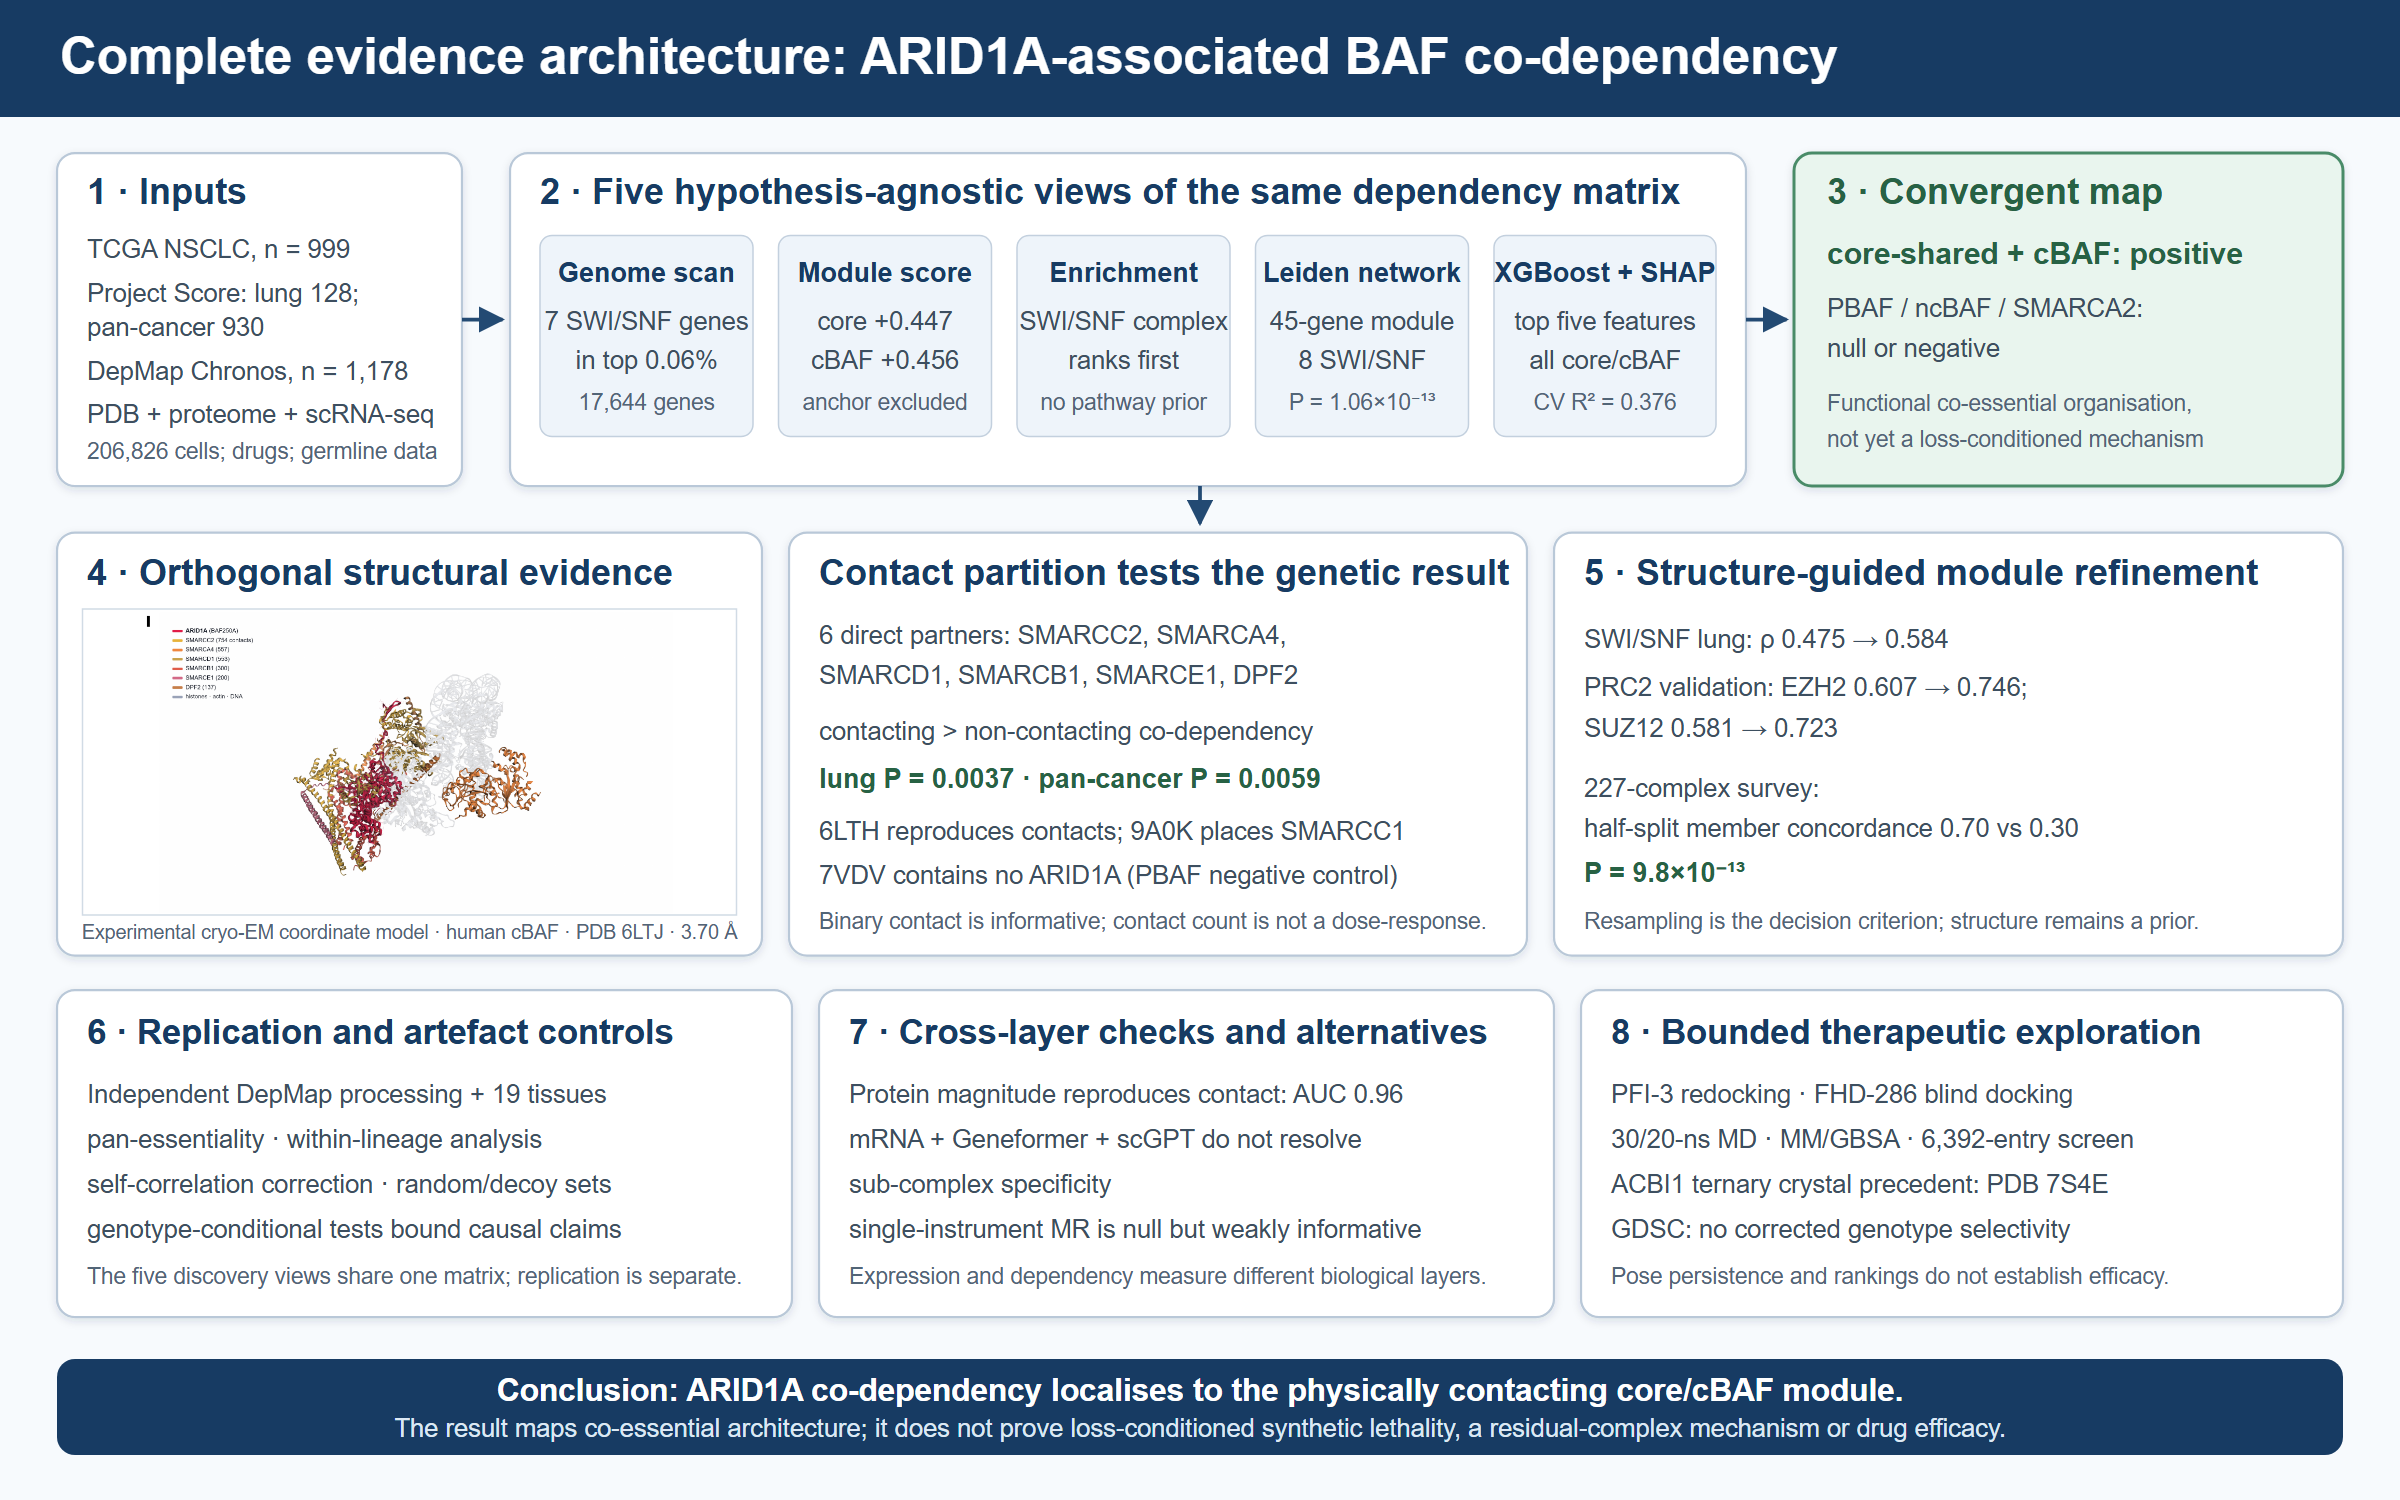
\includegraphics[width=0.82\linewidth]{Fig_workflow_complete.png}
\captionsetup{font=footnotesize}
\captionof{figure}{\textbf{Complete evidence architecture.} Five genome-scale
views converge on the core/cBAF module; experimental structure, module
refinement, replication and cross-layer checks then test and bound the result.
The structural thumbnail renders the experimentally determined cryo-EM
coordinate model (PDB 6LTJ), not a raw micrograph or density map. Therapeutic
analyses remain outside the primary evidence chain.}
\label{fig:workflow}
\end{landscape}

%==============================================================================
\section{Results}

\subsection{ARID1A is recurrently mutated and frequently truncated in NSCLC}

In the combined TCGA-LUAD and TCGA-LUSC cohort ($n = 999$) \citep{tcgaluad2014},
\gene{ARID1A} was mutated in \textbf{6.51\% of cases (65/999)}, at closely similar
frequencies in the two histologies (LUAD 6.23\%, 32/514; LUSC 6.80\%, 33/485;
Figure~\ref{fig:f1}a), establishing ARID1A as a recurrently altered gene in this
disease context.
The rate replicates outside TCGA: two independent lung adenocarcinoma cohorts
queried through the cBioPortal API \citep{cerami2012,gao2013} give 5.38\% (10/186,
MSK-IMPACT \citep{zehir2017}) and 6.67\% (177/2{,}653 \citep{lengel2023}) --- both
within a point of the TCGA estimate despite different platforms, populations and
ascertainment.

The mutational spectrum is that of a tumour suppressor (Figure~\ref{fig:f1}b): of
73 variants, \textbf{54.8\% (40/73) were truncating}, distributed without
hotspots, against $\sim$68\% for \gene{STK11} in the same cohort and almost
entirely hotspot missense for \gene{KRAS}. The spectrum is consistent with
frequent loss of function, although mutation status alone does not establish
complete loss of ARID1A protein in an individual model.

Stratifying TCGA-LUAD by \gene{ARID1A} expression tertile (low $n = 180$ versus
high $n = 180$), DESeq2 \citep{love2014} detected \textbf{501 significant genes}
(adjusted $P < 0.05$, $|\log_2\mathrm{FC}| > 1$; 421 up, 80 down;
Figure~\ref{fig:f1}c). This associative contrast establishes a transcriptional
context for low ARID1A expression but is not interpreted as a causal perturbation.

\begin{figure}[htbp]
\centering
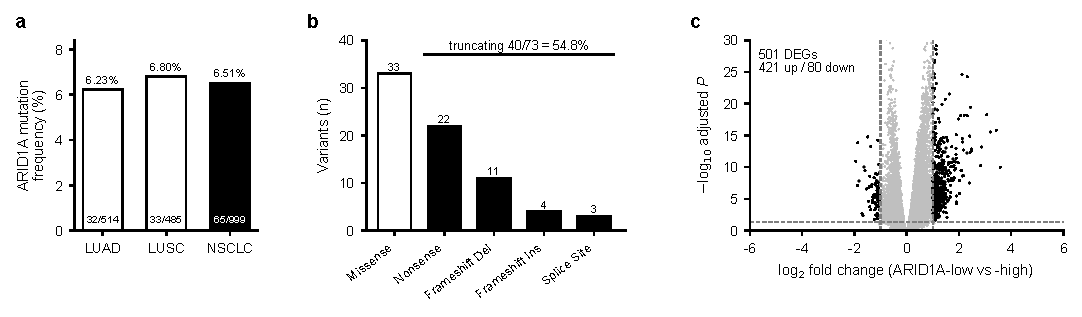
\includegraphics[width=\textwidth]{Fig1.pdf}
\caption{\textbf{ARID1A is recurrently mutated and frequently truncated in NSCLC.}
(\textbf{a}) Mutation frequency in TCGA-LUAD, TCGA-LUSC and the combined NSCLC
cohort; counts give mutated cases over cohort size. (\textbf{b}) Variant
classification spectrum; filled bars are truncating classes. (\textbf{c}) Volcano
plot of ARID1A-low versus ARID1A-high tertile differential expression; filled
points pass adjusted $P < 0.05$ and $|\log_2\mathrm{FC}| > 1$.}
\label{fig:f1}
\end{figure}

\subsection{Five methodologically distinct analyses converge on the ARID1A-associated BAF module}

Five analyses were run separately on the same dependency matrix; four of the
five use no complex composition at all
(Figure~\ref{fig:f2}). Supplementary Figure~S1 gives the sub-complex
compositions and the structure of the convergence argument.

\paragraph{Genome-scale scan.} Correlating the ARID1A dependency profile from the
Project Score screen \citep{behan2019,pacini2021} against $\sim$17{,}644 genes in
lung cancer ($n = 128$), the top-ranked genes were SMARCE1 (\#1, $\rho = 0.551$,
$P = 1.6\times10^{-11}$), SMARCB1 (\#2, 0.474), SMARCC1 (\#3, 0.380), DPF2 (\#4,
0.363), SMARCA4 (\#5, 0.357), ARID1B (\#7, 0.344) and SS18 (\#10, 0.313) --- seven
SWI/SNF subunits inside the top 0.06\% of the genome (hypergeometric enrichment in
the top 1\%: $P = 3.2\times10^{-12}$ lung, $5.5\times10^{-14}$ pan-cancer), while
PBAF- and ncBAF-specific subunits ranked in the bottom 90--97\%. The pan-cancer
ranking has the same shape (Supplementary Figure~S2): eight of the top nine genes
are SWI/SNF subunits, with the paralogue ARID1B only 32nd. A network-guided
druggability overlay places SMARCA4 first among co-dependencies for which a
chemical probe or clinical-stage inhibitor exists. This overlay prioritises
follow-up targets; it is not a compound--target--pathway network-pharmacology
analysis and does not establish genotype-selective efficacy.

\paragraph{Module scoring.} Core-shared and cBAF-specific modules were
significantly positive at both levels; PBAF-specific and alternative-ATPase
modules null; the ncBAF-specific module significantly negative pan-cancer
(Table~\ref{tab:mod}).

\begin{table}[htbp]
\centering
\caption{Complex-module co-dependency with ARID1A. The anchor is excluded from
every module (Section~\ref{sec:selfcorr}).}
\label{tab:mod}
\small
\begin{tabular}{lccccc}
\toprule
\textbf{Module} & \textbf{Subunits} & \textbf{Lung $\rho$} & \textbf{$P$}
 & \textbf{Pan-cancer $\rho$} & \textbf{$P$} \\
\midrule
Core-shared    & 8 & $+0.447$ & $1.2\times10^{-7}$ & $+0.461$ & $3.1\times10^{-50}$ \\
cBAF-specific  & 9 & $+0.456$ & $6.2\times10^{-8}$ & $+0.307$ & $1.0\times10^{-21}$ \\
PBAF-specific  & 4 & $-0.123$ & $0.166$            & $-0.012$ & $0.720$ \\
ncBAF-specific & 3 & $-0.157$ & $0.076$            & $-0.110$ & $8.1\times10^{-4}$ \\
Alt.\ ATPase (SMARCA2) & 1 & $-0.122$ & $0.170$    & $-0.002$ & $0.958$ \\
\bottomrule
\end{tabular}
\end{table}

\paragraph{Prior-free enrichment.} The top-100 co-dependent genes, submitted to
Enrichr \citep{xie2021} without context, returned SWI/SNF Complex (GO:0016514) as
the top term in lung (9/29 genes, adjusted $P = 1.5\times10^{-12}$), followed by
nBAF, CORUM EBAFb, npBAF and BAF --- every leading term a SWI/SNF sub-complex.

\paragraph{Co-essentiality community detection.} From 7{,}940 selectively
essential genes we built a genome-wide $k$-nearest-neighbour co-dependency graph
($K = 15$, $\rho > 0.15$) and ran Leiden community detection \citep{traag2019}
across a resolution sweep. At resolution 4.0 the ARID1A community contained
\textbf{45 genes including 8 SWI/SNF subunits} (hypergeometric
$P = 1.06\times10^{-13}$). The algorithm is given neither the anchor's identity
nor the study question.

\paragraph{Gradient boosting with SHAP.} Predicting ARID1A dependency from 3{,}000
genome-scale features (1{,}178 lines) gave cross-validated $R^2 = 0.376$. The top
five SHAP features \citep{lundberg2020} were SMARCB1, SMARCE1, SMARCC1, ARID1B and
DPF2, separated by a clear discontinuity from rank 6. PBAF/ncBAF subunits ranked
far lower (BRD9 \#30, ARID2 \#108, BRD7 \#224, PBRM1 \#301). Because the original
training driver was not retained, we performed a fully specified pre-submission
reanalysis with unsupervised variance-based feature selection and out-of-fold
prediction. It recovered the same five leading features and a similar
out-of-fold $R^2=0.390$, providing a reproducible sensitivity analysis rather
than relying on the historical model output alone.

\paragraph{Mandatory controls.} ARID1A is \emph{selectively}, not pan-, essential
--- dependent (gene effect $< -0.5$) in 15.4\% of lines and strongly dependent
($< -1.0$) in 1.3\% --- whereas pan-essential references are essential in 100\% of
lines, so its correlations cannot be a pan-essentiality artefact. Correspondingly
ARID1A co-dependency is strong with core BAF and null with every pan-essential
reference ($|\rho| \le 0.070$) and with PBRM1 ($+0.002$). Lung estimates are
computed within lineage; robustness to broader lineage composition is assessed
by separate within-tissue analyses across 19 tissues below.

\begin{figure}[htbp]
\centering
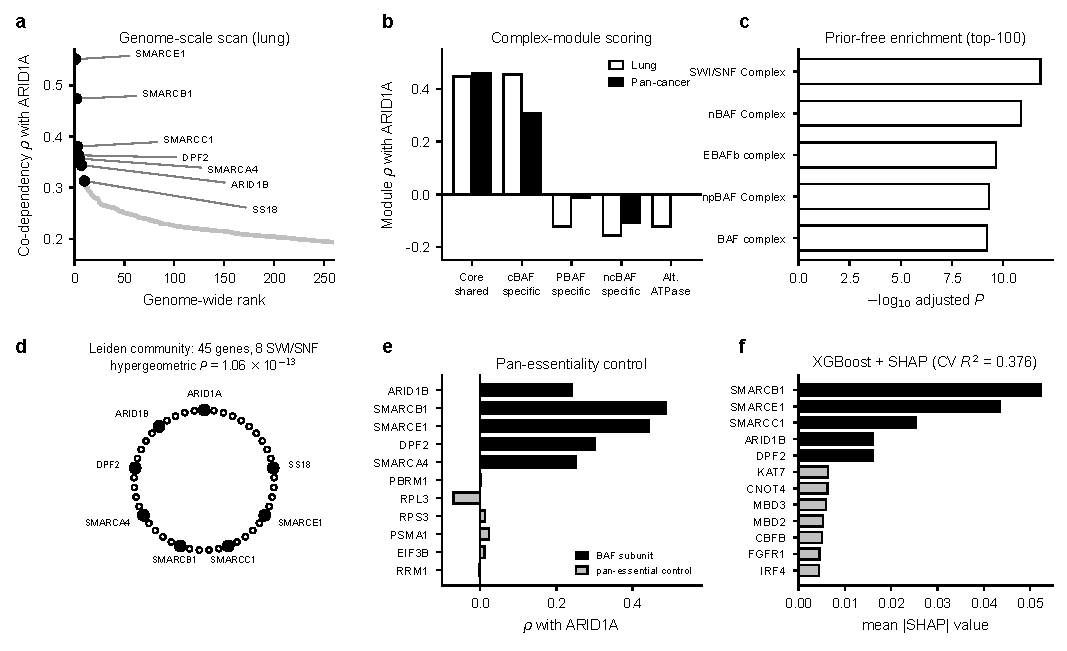
\includegraphics[width=\textwidth]{Fig2.pdf}
\caption{\textbf{Five methodologically distinct analyses converge.} (\textbf{a}) Genome-scale
co-dependency scan in lung cancer; SWI/SNF subunits are highlighted. (\textbf{b})
Complex-module scores in lung and pan-cancer. (\textbf{c}) Prior-free enrichment
of the top-100 co-dependent genes. (\textbf{d}) Leiden community containing
ARID1A. (\textbf{e}) Pan-essentiality specificity controls. (\textbf{f})
XGBoost/SHAP feature attribution.}
\label{fig:f2}
\end{figure}

\subsection{The experimental structure explains the genetic result and refines the
module definition}

The preceding section rests entirely on genetic correlation, so we introduced
evidence of an entirely different kind: the cryo-EM structure of the assembled
human BAF complex (PDB 6LTJ, 3.70\,\AA{}; base module 6LTH, 3.00\,\AA{})
\citep{he2020}, with the nucleosome-bound PBAF structure (PDB 7VDV)
\citep{yuan2022} as a
negative control --- it contains no ARID1A chain at all, confirming cBAF/PBAF
mutual exclusivity structurally rather than by assumption.

Parsing chain coordinates with Biopython \citep{cock2009}, ARID1A makes direct
heavy-atom contact (minimum distance 2.20--2.47\,\AA{}) with SMARCC2 (754 atom
pairs within 4.5\,\AA{}), SMARCA4 (557), SMARCD1 (553), SMARCB1 (300), SMARCE1
(200) and DPF2 (137), and no contact with ACTL6A (13.02\,\AA{}) or ACTB
(31.99\,\AA{}) (Figure~\ref{fig:structure}I). SMARCC2 is present as a homodimer
(chains N and O). Independent recomputation in the higher-resolution 6LTH gave
identical counts to within one atom pair. SMARCC1, unresolved in 6LTJ, contacts
ARID1A in the integrative model of the endogenous complex (PDB 9A0K; 186 pairs,
2.58\,\AA{}) \citep{mashtalir2020}; the two agree on all six subunits 9A0K models
to comparable depth, diverging only for SMARCE1 and DPF2, which it covers over 79
and 37 residues. We count SMARCC1 as contacting.

The wwPDB validation reports qualify how these coordinates should be used. The
full 6LTJ deposit has a low global map--model Q-score (0.007; 0.6th percentile
among same-resolution entries), whereas the independently deposited,
higher-resolution 6LTH base module has Q=0.526 (67.5th percentile). We therefore
use 6LTH as the primary replication of the interface rather than treating 6LTJ
alone as definitive. All six contact calls persisted in both deposits at 4.0,
4.5 and 5.0\,\AA{} and after removing the bottom decile of residue Q-scores
within every analysed chain (Supplementary Figure~S8b). The 196 ARID1A interface
residues were not selectively lower quality than non-interface ARID1A residues
in either deposit (two-sided Mann--Whitney $P=0.182$ for 6LTJ and $P=0.169$ for
6LTH). Thus the binary interface assignment is deposit- and threshold-robust,
although the low global quality of 6LTJ precludes stronger atom-by-atom
mechanistic claims.

\begin{figure}[p]
\centering
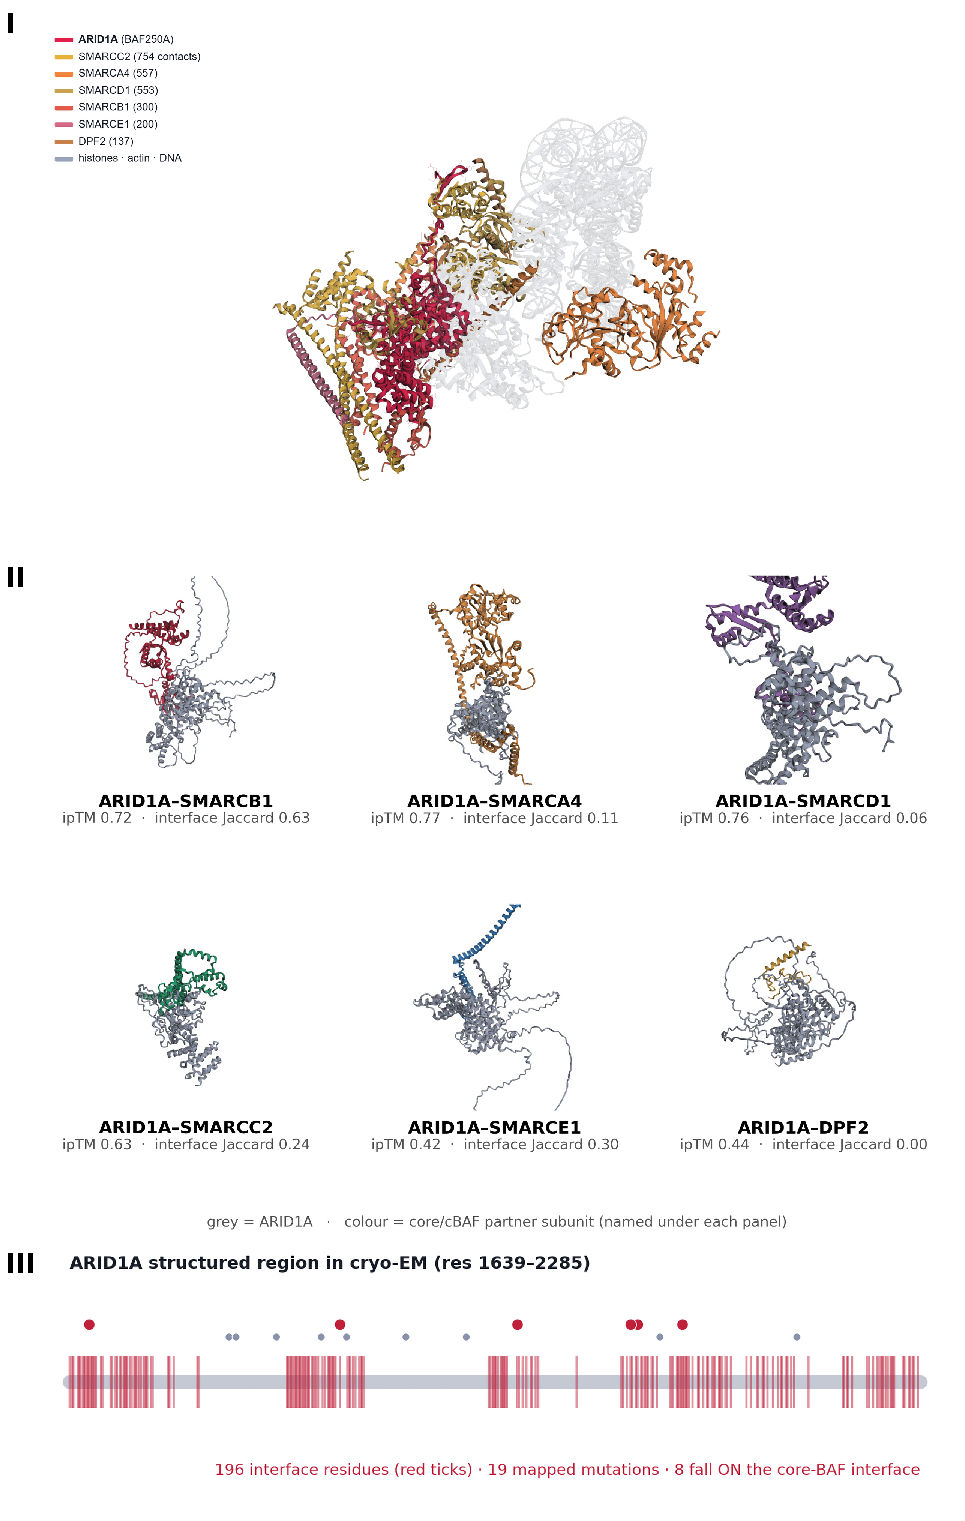
\includegraphics[width=0.80\textwidth]{FigM_structure.pdf}
\caption{\textbf{The ARID1A--core-BAF interface: experimental, predicted, and
mutated.} (\textbf{I}) ARID1A within the assembled human cBAF complex (PDB 6LTJ,
3.70\,\AA{}) \citep{he2020}, ARID1A in red, each contacting subunit coloured and
annotated with its heavy-atom contact count ($<$ 4.5\,\AA{}); histones, actin and
DNA grey. ARID1A contacts all six core/cBAF subunits at 2.20--2.47\,\AA{}, while
ACTL6A and ACTB lie 13.0 and 32.0\,\AA{} away. (\textbf{II}) The same six
complexes predicted by AlphaFold-Multimer \citep{jumper2021,evans2024,mirdita2022}
from sequence alone, with self-reported ipTM and Jaccard overlap against the
cryo-EM interface. The two highest-confidence models reproduce it worst; the best
reproduction ranks only third by ipTM. (\textbf{III}) The ARID1A region resolved
in 6LTJ (residues 1639--2285): red ticks are the 196 interface residues, circles
the 19 NSCLC mutations in this region, eight of them (filled) on the interface.}
\label{fig:structure}
\end{figure}

\paragraph{Physical contact separates stronger from weaker co-dependencies.}
Comparing the seven contacting genes against eight non-contacting or mutually
exclusive ones gave a lung median difference in $\rho$ of 0.436 (95\% bootstrap
interval 0.293--0.584; Cliff's $\delta=0.857$; exact two-sided Mann--Whitney
$P=0.0037$) and a pan-cancer difference of 0.314 (0.165--0.451;
$\delta=0.821$; $P=0.0059$). Restricted to the six subunits resolved in 6LTJ,
the group comparisons gave $P=0.0080$ and $P=0.0127$. This binary structural
partition is an orthogonal measurement to the genetic screen. It should not be
interpreted as a dose--response: among the six contacting subunits resolved in
the same structure, contact count was not positively associated with
co-dependency (lung Spearman $\rho=-0.657$, $P=0.156$; pan-cancer
$\rho=-0.600$, $P=0.208$). Physical contact is therefore used as a binary prior,
not as a quantitative predictor of dependency strength.

The group comparison was also insensitive to the contact definition
(Supplementary Figure~S8c). Excluding integrative-model-only SMARCC1 gave lung
and pan-cancer median differences of 0.432 (95\% bootstrap interval
0.162--0.590; exact $P=0.0080$) and 0.279 (0.090--0.471; $P=0.0127$),
respectively. All 15 leave-one-gene-out versions remained significant in each
cohort ($P<0.05$). Restriction to the eight subunits physically present in 6LTJ
retained the direction but, with only two non-contacting comparators, was
underpowered ($P=0.286$ in each cohort).

\paragraph{Curated module definitions are not optimal.} Restricting the core
module to the subunits the structure shows to contact the anchor gives a better
module: on DepMap (lung $n = 126$; pan-cancer $n = 1{,}178$) the correlation rises
from 0.475 to 0.584 (lung) and 0.499 to 0.533 (pan-cancer) while dropping two of
eight genes (Figure~\ref{fig:f3}c). ACTB and ACTL6A are individually null (lung
$\rho = 0.043$ and $0.122$) and act as dilution terms: in lung, leave-one-out over
those same eight (Figure~\ref{fig:f3}b) gains $+0.061$ and $+0.037$ on their
removal while removing a contacting subunit costs up to $-0.089$. The separation
is cleaner in lung than pan-cancer, where ACTL6A costs $-0.007$. SMARCD1 is an apparent exception --- despite the
second-largest interface its removal improves the pan-cancer score, matching its
null co-dependency ($\rho = -0.083$ lung, $-0.025$ pan-cancer). Separating the
paralogues resolves it: the dependency at that position runs through SMARCD2,
which no cBAF structure resolves ($\rho = +0.193$, $P = 2.9\times10^{-9}$
pan-cancer, tenth of 17{,}644 genes; $+0.184$, $P = 0.038$ in the smaller lung
panel). The structure localises the position, not the gene occupying it.

\paragraph{The refinement generalises to a second complex.} Repeating the
procedure on PRC2 with the cryo-EM structure of the human PRC2--AEBP2--JARID2
complex \citep{kasinath2018,kasinath2021} and two anchors
(Figure~\ref{fig:f3}d), both converge on the catalytic lobe EZH2--EED--SUZ12,
with the histone-chaperone subunits RBBP4 and RBBP7 removed: EZH2 improves from
0.607 to 0.746 and SUZ12 from 0.581 to 0.723. RBBP4/RBBP7 are shared with NuRD,
CAF-1 and SIN3, so their dependency profiles are driven by complexes other than
PRC2.

\paragraph{How far does structural contact go as a decision rule?} For two of the
three anchors it is exactly right: for ARID1A the contact-restricted core is the
best-performing definition, and for EZH2 the contact rule selects EED\,+\,SUZ12,
which an exhaustive subset search confirms is the optimum. For the third it is
not: RBBP4 makes a large, unambiguous contact with SUZ12 (685 heavy-atom pairs
across 61 interface residues) and would be retained, yet removing it improves the
module by a further $+0.092$. Membership in other complexes is the obvious
explanation, and it does not survive testing (Discussion).

\paragraph{Operational recommendation.} Structural contact is a good but imperfect
prior --- correct for two of three anchors --- and the criterion should be whether
the dropped member replicates on resampling, not the size of the gain, for the
reason given in the Discussion. The refinement is substantial and consistent:
$+0.109$ (SWI/SNF, lung), $+0.138$ (PRC2, EZH2) and $+0.142$ (PRC2, SUZ12) over
the curated definition.

\paragraph{The reproducibility criterion generalises beyond the two examples.}
We replaced the initial asymmetric survey with a fully nested, symmetric null
design (Supplementary Figure~S8a). For every split, both the anchor and the
member to drop were selected only in the discovery half and carried unchanged
into the held-out half; each curated complex was compared with two
size-matched random modules under the identical procedure. Of 277 eligible
human complexes, 266 yielded a paired comparison over 30 splits. Median held-out
drop-identity concordance was 0.60 for curated complexes and 0.333 for matched
null modules; the paired median difference was 0.25 (95\% bootstrap interval
0.175--0.308; one-sided paired Wilcoxon $P=1.03\times10^{-19}$; Cliff's
$\delta=0.425$). The held-out gain was positive in a median 0.933 of splits for
curated complexes and 0.767 for null modules. Thus the transferable result is a
nested reproducibility criterion for module refinement, not a universal rule
that non-contacting members should be removed.

\begin{figure}[htbp]
\centering
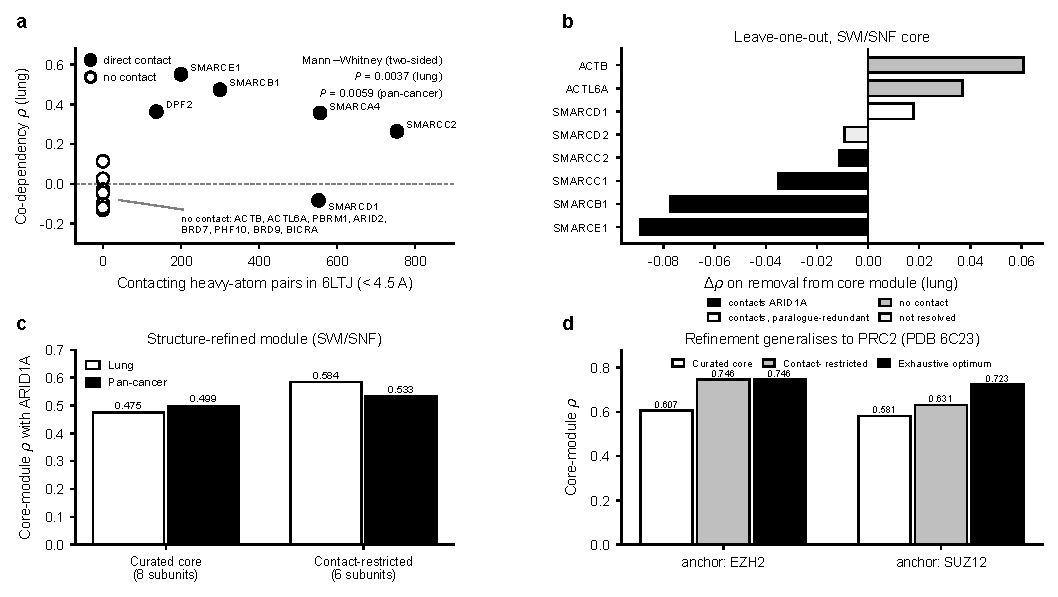
\includegraphics[width=\textwidth]{Fig3.pdf}
\caption{\textbf{The experimental structure explains and refines the genetic
result.} (\textbf{a}) Contacting heavy-atom pairs in PDB 6LTJ against co-dependency
$\rho$; filled points contact ARID1A directly. The inferential test compares
contacting with non-contacting subunits; contact count within the contacting group
does not show a positive dose--response. SMARCC1 is not plotted because
6LTJ does not resolve it; its contact is established in 9A0K. (\textbf{b}) Leave-one-out change in
the core-module correlation in lung, over the same eight subunits used in
(\textbf{c}), ordered by contact status; SMARCD2 is resolved in no cBAF structure
and so has no contact call. (\textbf{c}) Curated versus
contact-restricted core module in SWI/SNF. (\textbf{d}) The same refinement in PRC2
(PDB 6C23) for two anchors, against the exhaustive subset optimum.}
\label{fig:f3}
\end{figure}

\subsection{The continuous co-dependency pattern varies with ARID1A expression}

If co-dependency reflects shared complex state, its magnitude may vary with the
abundance of the anchor. Across \gene{ARID1A} expression quintiles the
core-module dependency changes strictly monotonically ($-0.706$ to $-0.510$ from
lowest to highest), as does the cBAF module, while PBAF ($\approx -0.19$) and
ncBAF ($\approx +0.01$) are flat. The trend is confined to the modules implicated
by the co-dependency analysis; partial correlation preserves the specificity
(pan-cancer core 0.411, $P = 3.6\times10^{-49}$; cBAF 0.218,
$P = 4.1\times10^{-14}$). Because expression is observational and does not
identify protein-null models, this gradient is a consistency analysis rather
than evidence of loss-induced sensitivity.

\subsection{Generalisation across tissues and independent replication}

Across 930 de-duplicated lines from 19 tissues, computed within each tissue,
SMARCB1 and SMARCC1 were positive in 19/19 tissues, DPF2 in 18/19, ARID1B 17/19
and SMARCA4 16/19, three to thirteen of them passing global Benjamini--Hochberg
correction \citep{benjamini1995}; PBRM1, ARID2 and SMARCA2 were each positive in
10/19 and negative in 9/19 with \emph{zero} significant tissues
(Figure~\ref{fig:f4}a).

Recomputation in a wholly different dataset and pipeline --- the DepMap 24Q4
Chronos gene-effect matrix, 1{,}178 lines \citep{depmap2025} --- reproduced the
pattern (Figure~\ref{fig:f4}b): core/cBAF positive, PBAF/ncBAF/alternative ATPase
null, so the finding is not an artefact of one processing pipeline.

\begin{figure}[htbp]
\centering
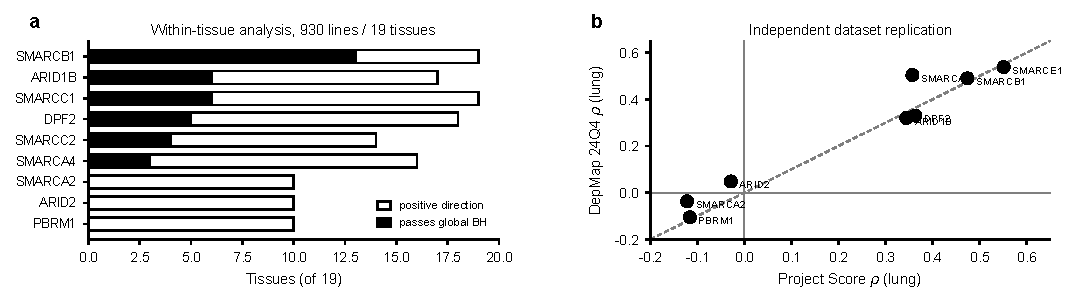
\includegraphics[width=\textwidth]{Fig4.pdf}
\caption{\textbf{Pan-cancer generalisation and independent replication.}
(\textbf{a}) Within-tissue co-dependency across 19 tissues; open bars count
tissues with a positive direction, filled bars those passing global BH correction.
(\textbf{b}) Project Score versus DepMap 24Q4 co-dependency in lung; the dashed
line is the identity.}
\label{fig:f4}
\end{figure}

\subsection{Genotype-conditional tests bound the co-dependency interpretation}

We next asked the distinct question of whether ARID1A-mutant cell lines are more
dependent on individual BAF subunits than wild-type lines. Across five tissues
with at least six mutant models, ARID1B had the expected direction in all five,
ARID2 and BRD9 in four, and the remaining subunits in one to three. None of the
65 tissue--subunit comparisons survived global Benjamini--Hochberg correction.
In lung ($n=6$ mutant, $n=122$ wild type), PBRM1 and ARID2 were nominally more
essential in mutant lines ($P=0.0217$ and $0.0248$), but both had $q=0.403$;
the principal contacting subunits were non-significant. Thus the continuous
co-dependency pattern is robust, whereas this dataset does not establish an
ARID1A-loss-conditioned vulnerability.

We therefore repeated the analysis using ARID1A protein abundance as the
primary state definition and mRNA abundance as a larger-sample sensitivity
definition. Gene effects were standardized within lineage before pooling, and
the bottom 5\%, 10\% and 15\% of ARID1A abundance were compared with the
remainder. The protein analysis included 535 usable lines (25, 52 and 80 in the
low groups); no individual subunit or prespecified BAF module passed
Benjamini--Hochberg correction at any threshold. At the protein bottom 10\%,
ARID1B was directionally more dependent (mean within-lineage $z$ difference
$-0.277$, 95\% bootstrap interval $-0.608$ to $+0.048$; $q=0.187$), whereas the
ARID1A-contacting module was directionally less dependent ($+0.152$,
$0.013$--$0.292$; $q=0.187$). The mRNA analysis gave the same corrected-null
conclusion. As an assay-dynamic-range control, the identical pooled design
strongly detected the established SMARCA4-low--SMARCA2 dependency: at the mRNA
bottom 10\%, $Delta z=-1.012$ ($-1.355$ to $-0.689$; $q=3.05\times10^{-9}$).
The negative ARID1A result is therefore not explained by an intrinsically
insensitive pooled pipeline (Supplementary Figure~S8d), but protein-defined
low abundance is still not equivalent to engineered biallelic loss.

\begin{figure}[htbp]
\centering
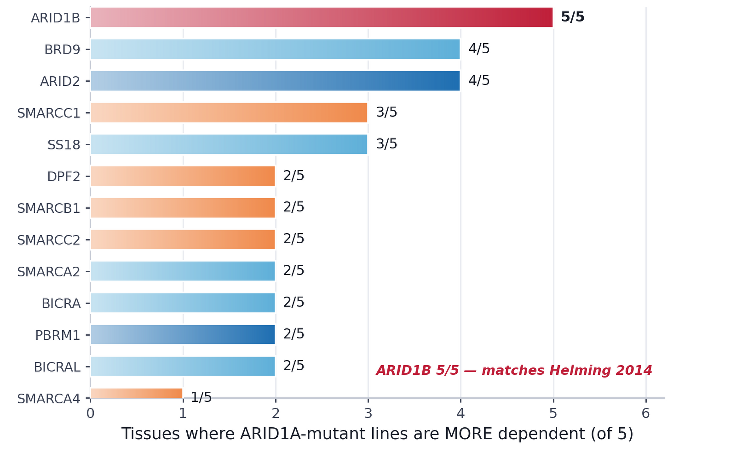
\includegraphics[width=0.72\textwidth]{Fig11_genotype.pdf}
\caption{\textbf{Genotype-conditional dependency is directional but
underpowered.} For each BAF subunit, the number of tissues (of five with
adequate sample size) in which ARID1A-mutant cell lines are more dependent than
wild-type lines. ARID1B has the expected direction in 5/5 tissues, but no
tissue--subunit comparison survives global multiple-testing correction. This
analysis measures a different axis from the continuous co-dependency gradient
and is reported as a boundary on interpretation, not as evidence of synthetic
lethality.}
\label{fig:genotype}
\end{figure}

\subsection{A self-correlation artefact must be corrected}
\label{sec:selfcorr}

Module scoring correlates an anchor's dependency against a module mean. If the
anchor is itself a member, $1/k$ of the module score \emph{is} the anchor. Across
three complexes and 48 anchor--module pairs all 48 were inflated by more than
0.10, with inflation scaling inversely with module size (Spearman
$\rho = -0.597$, $P = 7.3\times10^{-6}$; mean $+0.506$ at $k = 2$, $+0.358$ at
$k = 3$, $+0.197$ at $k = 9$). At small $k$ the consequence is a reversed
conclusion, not a shifted estimate: STAG2 appears strongly co-dependent with its
own cohesin module ($+0.839$) when the anchor-excluded value is $-0.045$, not
significantly different from zero. All analyses here exclude the anchor from
every module.

That correlating a variable with a mean containing it inflates the correlation is
elementary; the contribution here is the empirical magnitude and the
demonstration that at small $k$ it reverses conclusions. We have not surveyed how
often the anchor is left in, and make no claim about prevalence.

\paragraph{Benchmark with the correction applied.} The shared core module is
common to all sub-complexes, so a high core score is expected for \emph{every}
anchor; the testable hypothesis is one of discrimination. Scored over fourteen
anchors of known mutually exclusive membership across SWI/SNF and PRC2, all
fourteen are assigned correctly, competing modules near zero or negative
throughout, and SMARCA2 returns null on all four modules ($|\rho| \le 0.042$) ---
correct for an alternative ATPase belonging to no sub-complex. Since
co-essentiality recovering complex membership is established
\citep{pan2018,wainberg2021}, this is a positive control, not a novel finding.

\paragraph{Null controls.} Three hundred random genes outside the complex give a
best exclusive-module correlation of $+0.028$ (median; 95th percentile $+0.095$);
only 4.0\% pass a $\rho > 0.1$ threshold and only 0.3\% exceed the weakest true
anchor (Mann--Whitney $P = 1.7\times10^{-7}$). Decoy anchors from unrelated
complexes give a median of $+0.091$, but not all are inert: MED12 scores $+0.241$
on ncBAF and the three PRC2 core subunits lean toward ncBAF ($+0.138$ to
$+0.181$). Thresholds in the 0.1--0.25 range therefore admit false positives from
functionally related complexes, and assignments should carry their margin over
the best competitor.

\subsection{Computational structural methods cross-validate one interface, and one
confidence metric fails}

Blind rigid-body docking \citep{jimenez2018} with 200 swarms (6{,}000 poses per
partner) located the correct interface for all four partners tested (best Jaccard
0.325--0.500; Figure~\ref{fig:f5}a). Top-ranked poses perform poorly because the
scoring function ranks large scaffold interfaces badly, so we treat this only as
evidence that the interface is findable.

AlphaFold-Multimer \citep{jumper2021,evans2024,mirdita2022} run from sequence alone
accurately recovered the ARID1A--SMARCB1 interface (87\% recall, Jaccard 0.628).
But across the six partners \textbf{ipTM and interface recovery are unrelated}
(Spearman $\rho = -0.14$, $P = 0.79$; Figure~\ref{fig:f5}b), and the two
highest-confidence predictions are among the worst reproductions, consistent with
benchmarking showing that multimer confidence metrics degrade for large and
asymmetric assemblies \citep{zhu2023af,bibppi2023} and with the incomplete
structural coverage of the human interactome \citep{bibinteractome}. ipTM should
not be used as a reliability filter when validating interfaces within large
assemblies. The six models are shown in Figure~\ref{fig:structure}II.

The interface is also where a substantial share of the mutations fall: of the 73
ARID1A mutations in the NSCLC cohort, 19 lie within the region resolved in 6LTJ
(residues 1639--2285) and eight of those land on the 196-residue core-BAF contact
surface (Figure~\ref{fig:structure}III). Because most ARID1A mutations are
truncating (Figure~\ref{fig:f1}b) and remove the region entirely, this is not
evidence for a separable interface-disrupting mutation class; it records only
that the contact surface lies within the mutated territory.

\begin{figure}[htbp]
\centering
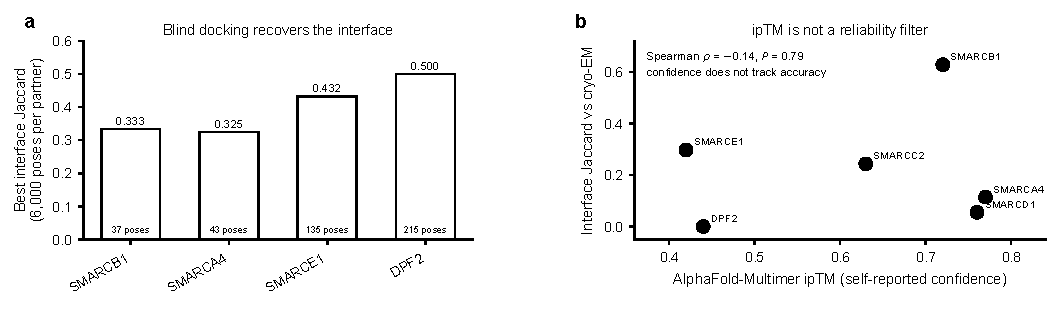
\includegraphics[width=\textwidth]{Fig5.pdf}
\caption{\textbf{Computational structural cross-validation.} (\textbf{a}) Blind
docking interface recovery; the best Jaccard over all 6{,}000 poses per partner,
with the number of near-native poses ($J \ge 0.2$) annotated. (\textbf{b})
AlphaFold-Multimer interface reproduction against self-reported ipTM for the six
contacting partners.}
\label{fig:f5}
\end{figure}

\subsection{Alternative explanations excluded}

\paragraph{The complex the dependency targets is expressed in real tumours.} In
206{,}826 Harmony-integrated cells from a NSCLC single-cell atlas
\citep{kim2020,korsunsky2019}, ARID1A and the residual core/cBAF subunits are
expressed in the malignant epithelial compartment (Supplementary Figure~S3).
To respect the nesting of cells within specimens, we aggregated the 35{,}600
epithelial cells to 48 sample-level observations. Mean ARID1A expression was
modestly associated with the mean core/cBAF score (Spearman $\rho=0.416$,
$P=0.0033$); samples below versus above the median differed by only 0.0147 score
units (medians $-0.0179$ versus $-0.0032$; exact Mann--Whitney $P=0.0257$).
The small sample-level effect shows that the genes are detectable in tumour
epithelium but does not establish that low ARID1A expression is functional loss
or that an intact residual complex persists. Human Protein Atlas
immunohistochemistry agrees at the
protein level, reporting moderate-to-strong nuclear ARID1A and strong nuclear
SMARCB1 and SMARCA4 staining across malignant tissue including lung
\citep{hpa2015}.

\paragraph{Transcript-level data cannot resolve complex specificity.} \emph{In
silico} deletion of ARID1A with a single-cell foundation model
\citep{theodoris2023} in 7{,}270 malignant epithelial cells \citep{kim2020}
returned null for BAF subunit ranks ($P = 0.3$--$0.6$) in two independent runs;
the undownsampled run increased detection counts three- to four-fold and remained
null. An architecturally different foundation model agrees from the opposite
direction: in scGPT's representation \citep{cui2024} the SWI/SNF subunits sit
close to ARID1A regardless of sub-complex, with PBRM1 its nearest SWI/SNF
neighbour despite a genetic PBAF co-dependency of essentially zero
(Supplementary Figure~S3). Bulk mRNA and
cell-line proteomic correlations \citep{goncalves2022} likewise place ARID1A in
positive correlation with \emph{all thirteen} BAF family genes, including the
mutually exclusive PBRM1 and SMARCA2 (Figure~\ref{fig:f6}a), so a conclusion
about complex specificity drawn from the sign of an expression correlation would
be demonstrably wrong at the genetic level.

\paragraph{The specificity is present at the protein layer but not the transcript
layer.} Sign is not the informative feature; magnitude is. On the 677 cell lines
carrying both measurements, the same lines used for both, whether ARID1A contacts
a subunit is invisible in the transcriptome (median $\rho$ 0.571 contacting
versus 0.432 not; AUC 0.57, $P = 0.69$) and plainly visible in the proteome
(0.598 versus 0.207; AUC 0.96, $P = 0.0012$), where the correlation also tracks
interface size ($\rho = +0.65$, $P = 0.0086$, against $+0.18$, $P = 0.53$ for
transcripts). The comparison is confounded: protein correlation tracks detection
rate and abundance ($\rho = +0.82$ for both) and contacting subunits are the
better-measured ones. Restricted to the nine subunits detected in over 90\% of
lines the protein-level difference persists (0.605 versus 0.385, $P = 0.048$)
while the transcript-level difference stays absent and reverses in sign, so we
report the contrast as supported but abundance-limited.

An exploratory Mendelian-randomization analysis did not provide evidence for a
germline ARID1A-expression effect on lung-cancer risk (Figure~\ref{fig:f6}b).

\begin{figure}[htbp]
\centering
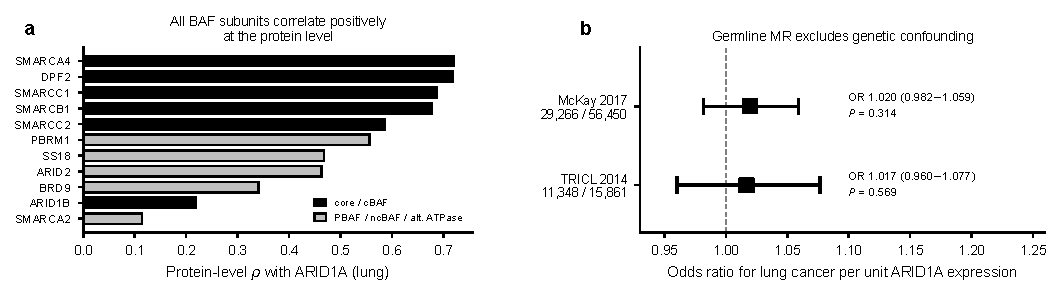
\includegraphics[width=\textwidth]{Fig6.pdf}
\caption{\textbf{Expression-layer comparison and exploratory germline analysis.} (\textbf{a}) Protein-level
correlation of ARID1A with BAF family subunits in lung cell lines; all subunits
correlate positively regardless of sub-complex membership. (\textbf{b}) Two-sample
Mendelian randomization \citep{hemani2018} using ARID1A \emph{cis}-eQTL
instruments \citep{vosa2021} against two independent lung cancer GWAS
\citep{mckay2017}; squares are odds ratios with 95\% confidence intervals. Both
are null ($\mathrm{OR} = 1.020$, $P = 0.314$; $\mathrm{OR} = 1.017$,
$P = 0.569$). Only one non-lung instrument was available: ARID1A carries seven independent
\emph{cis}-eQTLs across 49 GTEx tissues \citep{gtex2020} and none in lung, as
expected for a haploinsufficient tumour suppressor under purifying selection
\citep{karczewski2020}. The null estimates are therefore weakly informative and
cannot exclude genetic confounding.}
\label{fig:f6}
\end{figure}

\subsection{Pharmacological data do not establish genotype selectivity}

Thirteen GDSC compounds targeting PARP, ATR, ATM, EZH2 or SWI/SNF were compared
between ARID1A-mutant and wild-type models in lung and pan-cancer strata. No
comparison survived within-stratum Benjamini--Hochberg correction ($q\ge0.27$).
PFI-3 and I-BRD9 were among the least active compounds in the lung panel (mean
AUC 0.977 and 0.956), leaving little dynamic range for a genotype interaction.
These data are therefore uninformative rather than evidence against selectivity.
Likewise, genotype-conditional CRISPR effects for SMARCA4 and SMARCA2 did not
survive correction. The present study consequently makes no therapeutic-efficacy
claim: co-dependency prioritizes functional relationships, not drug targets, and
requires protein-loss-defined or isogenic validation before pharmacological
translation.

As a bounded structural-plausibility check, redocking PFI-3
\citep{fedorov2015} into its crystallographic SMARCA2/4 bromodomain pocket (PDB
5DKC) with AutoDock Vina \citep{eberhardt2021} reproduced the deposited pose at
0.48\,\AA{} RMSD and gave a score of $-8.4$\,kcal\,mol$^{-1}$
(Figure~\ref{fig:docking}A,B; Supplementary Figure~S4). Blind docking of the
clinical-stage dual SMARCA2/4 ATPase inhibitor FHD-286 \citep{fhd286trial2025}
into PDB 7VDT gave $-9.17$\,kcal\,mol$^{-1}$ (Figure~\ref{fig:docking}A;
Supplementary Figure~S6). No
public co-crystal validates that pose, however, and neither docking score is a
measured affinity or evidence of ARID1A-genotype selectivity. As a secondary
pose-persistence check, one explicit-solvent trajectory per complex was analysed
(Supplementary Figure~S5). Pocket-fitted ligand RMSD was $1.75 \pm 0.88$\,\AA{}
for PFI-3 over 30\,ns and $2.21 \pm 0.21$\,\AA{} for FHD-286 over 20\,ns;
the corresponding binding-site backbone RMSD values were $0.54 \pm 0.13$ and
$1.33 \pm 0.16$\,\AA{}. Single-trajectory MM/GBSA endpoint estimates were
$-27.93 \pm 2.33$ and $-33.45 \pm 4.29$\,kcal\,mol$^{-1}$, respectively.
These framewise summaries show bounded behaviour within the sampled
trajectories only. They do not validate the blind-docked FHD-286 pose, estimate
absolute affinity or establish genotype selectivity, and remain outside the
primary evidentiary chain.

Not every tractability argument rests on a predicted pose. The ACBI1 ternary
complex has been resolved experimentally by X-ray diffraction (PDB 7S4E,
2.25\,\AA{}), directly showing engagement of the human SMARCA2 bromodomain by
ACBI1 together with VHL--ElonginC--ElonginB \citep{dixon2022}. We did not redock
or resimulate that deposited complex. It provides a structural precedent for
ligandable SMARCA2 engagement and targeted degradation, but it does not establish
that ARID1A-deficient cells are selectively sensitive to ACBI1 or to any other
SMARCA2/4-directed agent.

An archived AutoDock Vina screen of a 6{,}392-entry project compound library was
also recovered and audited (Supplementary Figure~S7). Within the project's
$-13$ to $-5$\,kcal\,mol$^{-1}$ artefact-exclusion window, 5{,}311 bromodomain
and 5{,}493 ATPase scores remained. YM-750, arcyriaflavin~A and BINA led the
bromodomain ranking; MK-3207, BT-11 and SR-1664 led the ATPase ranking. The run
was resumed at lower exhaustiveness and the exact library source/version
metadata were not retained, so the result is reported only as a ranking
sensitivity analysis. These scores are neither binding affinities nor evidence
that the compounds are repurposing candidates.

\begin{figure}[p]
\centering
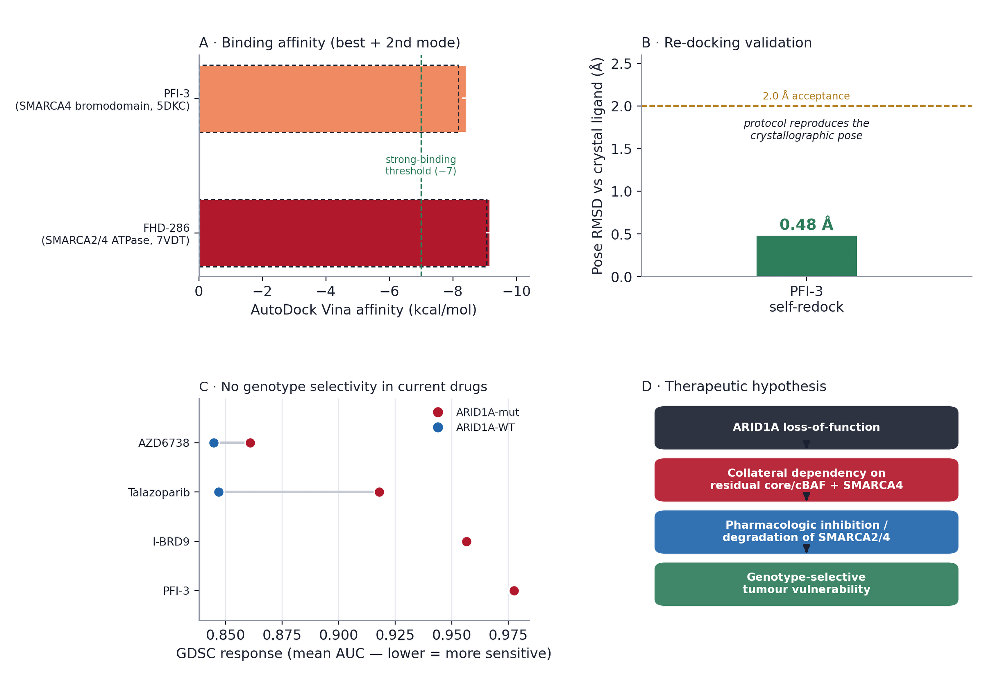
\includegraphics[width=0.92\textwidth]{Fig8_docking.pdf}
\caption{\textbf{Exploratory target-engagement plausibility does not establish
ARID1A-genotype selectivity.} (\textbf{A}) AutoDock Vina scores for PFI-3 in the
SMARCA2/4 bromodomain (PDB 5DKC) and FHD-286 in the SMARCA4 ATPase nucleotide
pocket (PDB 7VDT); dashed outlines mark the second-ranked mode.
(\textbf{B}) Positive-control redocking reproduces the PFI-3 crystallographic
pose at 0.48\,\AA{} RMSD. (\textbf{C}) Representative GDSC responses stratified
by ARID1A genotype. None of the thirteen tested compounds survived
within-stratum Benjamini--Hochberg correction; PFI-3 and I-BRD9 were near the
inactive end of the lung panel, limiting the ability to detect an interaction.
(\textbf{D}) Bounded therapeutic hypothesis linking ARID1A loss, collateral BAF
dependence and pharmacological inhibition. Panels A, B and D are exploratory:
docking scores rank modelled poses rather than measuring binding affinity, and
the diagram is a hypothesis rather than an efficacy claim.}
\label{fig:docking}
\end{figure}

%==============================================================================
\section{Discussion}

Five methodologically distinct analyses of one CRISPR dependency matrix converge
on core-shared and cBAF-associated subunits. The pattern survives
pan-essentiality and lineage controls, is reproduced in a second processing
resource and across 19 tissues, and aligns with a binary contact partition in an
experimental structure. Together these results map co-essential organization of
the ARID1A-associated BAF module. They do not show that ARID1A loss creates the
pattern, because mutation-, protein- and mRNA-defined conditional analyses are
non-significant after correction even though the pooled design detects a known
paralogue-dependency positive control.

\paragraph{Curated module definitions can be tested empirically.} The
266-complex nested survey shifts the methodological emphasis from maximizing an
in-sample correlation to reproducing the identity of a dilutive member in
held-out data. Applying the same discovery-half anchor and drop selection to
curated and matched-null modules removes the main selection asymmetry of the
initial survey; the paired concordance advantage remains large. This criterion
is useful beyond SWI/SNF, while remaining a statistical refinement rather than
proof that the nominated member is biologically dispensable.

\paragraph{Structure is a prior, not a rule.} We expected structural contact to
supply the decision criterion. In SWI/SNF the prior happens to be correct,
because the two dilutive subunits are also the two non-contacting ones; PRC2
dissociates the properties, since RBBP4 contacts SUZ12 substantially yet dilutes.
Subunit promiscuity is the obvious candidate, and it fails: the number of curated
human complexes containing each subunit \citep{meldal2022} --- an external count,
not one derived from the dependency data --- does not predict the leave-one-out
delta (Spearman $\rho = +0.21$, $P = 0.63$ within SWI/SNF), and dilutive and
load-bearing subunits have indistinguishable counts ($P = 0.91$). Curation depth
confounds such counts, so this bounds rather than closes the question. We say so
explicitly because the purely structural rule would be the more attractive claim
and is not what our data support.

\paragraph{Two layers that do not substitute for one another.} Every BAF family
gene correlates positively with ARID1A in both mRNA and protein, mutually
exclusive subunits included, so the sign of an expression correlation carries no
information about complex identity. What separates the layers is that the
protein-level magnitude reproduces the structural partition while the
transcript-level magnitude does not --- an orthogonal measurement type, on the
same cell lines, recovering what the CRISPR screens give. Transcriptional
co-regulation is a poor proxy for complex membership; protein abundance is a
usable one, within the limits of what mass spectrometry detects.

\paragraph{Relationship to existing paradigms.} ARID1B shows a \emph{positive}
continuous co-dependency with ARID1A, superficially opposite to synthetic
lethality \citep{helming2014}, and is robust across pipelines. In the separate
genotype-stratified analysis ARID1B had the expected direction in all five
tissues, and the protein- and mRNA-defined pooled analyses also pointed toward
greater ARID1B dependency, but no comparison survived multiplicity correction.
The same pooled pipeline recovered the SMARCA4-low--SMARCA2 positive control, so
the corrected-null ARID1A result is biologically informative rather than a
generic lack of assay sensitivity. It is compatible with the established
ARID1A--ARID1B relationship but does not independently reproduce it. More
broadly, continuous co-dependency
across heterogeneous lines and conditional essentiality after complete loss are
different estimands. Protein-defined null models or isogenic perturbations are
needed before translating the former into a synthetic-lethal claim.

\paragraph{Relationship to residual-complex compensation.} In dedifferentiated
endometrial carcinoma, ARID1A/ARID1B deficiency has been shown to reduce cBAF
while increasing the biochemical abundance and chromatin activity of ncBAF and
PBAF, accompanied by sensitivity to disruption of residual complexes
\citep{stlaurent2025}. Our continuous co-dependency map points in a different
direction: core/cBAF-associated subunits are positive, whereas the defining
PBAF/ncBAF subunits are null or negative. The two results need not conflict.
The endometrial study measures a loss-conditioned change in complex abundance and
function in a defined tumour state; we measure baseline co-essential covariance
across heterogeneous cell lines. The apparent contrast is therefore a testable
context and estimand difference, not evidence that either layer substitutes for
the other.

%==============================================================================
\section*{Limitations of the study}
\addcontentsline{toc}{section}{Limitations of the study}

The study is entirely computational and correlative. Positive co-dependency
identifies cell lines in which two genes tend to be essential together; it does
not establish that loss of one gene creates dependence on the other. The
mutation-defined genotype tests were underpowered and non-significant after
correction. Protein- and mRNA-defined low-abundance analyses used more lines and
an internally validated pooled design but likewise yielded no corrected module
dependency; abundance tails do not guarantee biallelic loss or absence of
residual protein. Isogenic perturbations and rescue experiments remain the
necessary next tests of loss-conditioned vulnerability.

The structural contact analysis supplies an orthogonal physical rationale rather
than a mechanism. The full 6LTJ model has a poor global wwPDB Q-score relative
to same-resolution entries; the binary interface is supported by the
higher-quality 6LTH replicate, distance-threshold sensitivity and residue-Q
filtering, but fine atom-level interpretation of 6LTJ is not warranted. The
analysis uses static wild-type assemblies and therefore cannot show
the composition or conformation of a residual complex after ARID1A loss. Contact
status separates the co-dependency groups, but contact count does not show a
positive dose--response among resolved contacts. Co-immunoprecipitation or
native-gel assays would be needed to test complex integrity directly.

Module refinement is characterised mechanistically on two complexes and three
anchors and surveyed statistically across 266; the symmetric nested survey
establishes held-out reproducibility of the nominated member relative to a
matched null, not that dropping it is biologically correct, and the mechanism is
unresolved.
Two subunits are placed by an integrative model rather than refined density:
SMARCC1, which no experimental cBAF structure resolves, and SMARCD2, whose
position is inferred from its paralogue. Computational structural methods
validate only the ARID1A--SMARCB1 interface effectively; the 14/14 discrimination
benchmark is a positive control rather than a novel finding, and decoy controls
are not fully inert. The five discovery analyses share one dependency matrix and
are methodologically distinct rather than biologically independent. The
single-cell result is sample-aggregated but remains an expression analysis, and
the transcript- and foundation-model negatives are unexplained mechanistically.
The molecular-dynamics analyses comprise one short trajectory per complex;
their framewise variation is not uncertainty across independent simulations.
Moreover, MM/GBSA omits conformational entropy and FHD-286 starts from a
blind-docked rather than crystallographic pose. These analyses test persistence
of the modelled poses over the sampled windows, not pose correctness, absolute
binding affinity or therapeutic efficacy. The recovered virtual screen combines
an initial run at Vina exhaustiveness 8 with a resumed run at exhaustiveness 4,
and its exact compound-library source/version metadata were not archived.
Consequently its ranks are exploratory, are not directly comparable to a
uniform-exhaustiveness screen and cannot support repurposing claims.

%==============================================================================
\section*{Methods}
\addcontentsline{toc}{section}{Methods}

\paragraph{Data sources.} TCGA-LUAD ($n = 514$) and TCGA-LUSC ($n = 485$)
\citep{tcgaluad2014}; the Sanger Project Score CRISPR screen, de-duplicated by
model identifier (lung $n = 128$; pan-cancer 930 lines, 19 tissues)
\citep{behan2019,pacini2021}; the DepMap 24Q4 Chronos matrix (1{,}178 lines)
\citep{depmap2025}; PDB 6LTJ, 6LTH, 6C23 and 9A0K; GEO GSE131907
\citep{kim2020}; OpenGWAS accessions for the eQTL exposure \citep{vosa2021} and
lung cancer outcomes \citep{mckay2017}.

\paragraph{Mutation landscape and differential expression.} maftools
\citep{mayakonda2018} on the clinically matched cohort denominator; other MAF
sources give slightly different denominators (6.1--6.8\%), so the cohort
definition must be stated for reproduction. DESeq2 \citep{love2014} on TCGA-LUAD
by \gene{ARID1A} expression tertile, significance at adjusted $P < 0.05$ and
$|\log_2\mathrm{FC}| > 1$.

\paragraph{Independent mutation-frequency replication.} Two non-TCGA lung
adenocarcinoma cohorts queried through the cBioPortal REST API
\citep{cerami2012,gao2013}: \texttt{luad\_mskimpact\_2021} ($n = 186$)
\citep{zehir2017} and \texttt{luad\_mskcc\_2023\_met\_organotropism}
($n = 2{,}653$) \citep{lengel2023}. A sample was called mutant if it carried at
least one non-synonymous \gene{ARID1A} variant; frequency is mutant over all
sequenced samples. Both are targeted panels covering ARID1A, ARID1B, SMARCA4,
SMARCB1, SMARCD1, PBRM1 and ARID2 (SMARCE1 and SMARCA2 added in v505), which is
why the replication is restricted to mutation frequency.

\paragraph{CRISPR co-dependency.} Spearman correlation with global
Benjamini--Hochberg correction \citep{benjamini1995}. \textbf{Tissue-level
correlations are computed within tissue}; pan-cancer values are pooled, the
lineage control being the separate 19-tissue analysis. Module score is the mean
gene effect over module members, \textbf{with the anchor excluded from every
module}. Table~\ref{tab:mod} uses Project Score; the refinement and leave-one-out
analyses use DepMap 24Q4, which is why the curated core's correlation differs
between them. Prior-free
enrichment via Enrichr \citep{xie2021} on the top-100 co-dependent genes only.
Co-essentiality network from 7{,}940 selectively essential genes with Leiden
community detection \citep{traag2019}, community identity interpreted only after
detection. The archived feature-attribution analysis used XGBoost with SHAP
\citep{lundberg2020}. For reproducible sensitivity analysis, the DepMap 24Q4
matrix was restricted to the 3{,}000 non-target genes with highest variance,
missing values were median-imputed, and prediction was evaluated by five-fold
out-of-fold cross-validation (shuffle seed 20260831). XGBoost used 500 trees,
maximum depth 3, learning rate 0.03, subsample and column-sample fractions 0.8,
and $L_2$ regularisation 1.0; SHAP values were then computed from a model fitted
to all 1{,}178 lines. Null controls: 300 random non-member genes and 13 decoy
anchors from PRC2, cohesin, ribosome, proteasome, RNA polymerase II and Mediator,
scored identically.

\paragraph{Structural analysis.} Biopython \citep{cock2009} parsing of PDB 6LTJ
and 6LTH (SWI/SNF) and 6C23 (PRC2); minimum heavy-atom distance and count of
heavy-atom pairs within 4.5\,\AA{} between the anchor chain and every other chain;
chain identity verified against PDB COMPND records; exact two-sided
Mann--Whitney comparison of contacting versus non-contacting groups, with
Cliff's delta and a 20{,}000-resample percentile bootstrap interval for the
median difference (seed 20260831);
Spearman correlation of contact count with co-dependency was assessed separately
among the six contacts resolved in 6LTJ. Leave-one-out and
exhaustive-subset module recomputation. In 6C23 subunits are modelled as disjoint
fragments rather than separate copies, so per-gene contacts are summed across
fragments and a contact required at least three interface residues. The same
criterion placed SMARCC1 using the integrative model 9A0K \citep{mashtalir2020};
built from crosslinking mass spectrometry and electron-microscopy envelopes
rather than refined density, it is used only for the binary contact call, and
modelled residue coverage was compared subunit by subunit first. Subunit promiscuity was the number of EBI Complex Portal
complexes containing that protein \citep{meldal2022}, tested against the
leave-one-out delta by Spearman correlation.

\paragraph{Structure-quality and contact-call sensitivity.} Official wwPDB
validation XML reports and deposited mmCIF coordinates were parsed for 6LTJ and
6LTH. We extracted resolution, EMDB accession, global and chain Q-scores,
same-resolution percentiles, atom inclusion, clashscore, Ramachandran outliers
and rotamer outliers. Heavy-atom contacts were recomputed at 4.0, 4.5 and
5.0\,\AA{}. To test sensitivity to locally weak model support, residues in the
bottom decile of wwPDB residue Q-score were removed separately within each
analysed chain before contact calls were repeated. Interface versus
non-interface ARID1A residue Q-scores were compared by two-sided Mann--Whitney,
and shared ARID1A residues were compared between deposits by paired Wilcoxon.
Structural genetic-group sensitivity used exact two-sided Mann--Whitney,
Cliff's delta and 20{,}000-resample percentile bootstrap intervals (seed
20260901) for the original, experimental-contact-only and
physically-present-subunit definitions, plus leave-one-gene-out analyses.

\paragraph{Protein versus transcript layer.} Sanger cell-line proteomics
\citep{goncalves2022} and CCLE expression were matched through Cell Model
Passports identifiers, giving 677 lines with both. Per subunit, the ARID1A-partner
Spearman correlation was computed at the protein and the transcript level on the
identical lines, so sample composition cannot generate a difference between
layers, and the contacting and non-contacting groups compared within each layer by
two-sided Mann--Whitney. Because protein correlation is not independent of how
well a protein is measured, detection rate and abundance were tested as
confounders and the comparison repeated on subunits detected in over 90\% of
lines.

\paragraph{Generalisation survey.} Complex Portal human complexes containing
6--21 DepMap-covered subunits were eligible (277). In each of 30 random
half-splits, the highest-correlating anchor and the member whose removal most
improved the anchor-excluded module score were selected using only the discovery
half, then carried unchanged into the held-out half. Two random gene modules
matched to each complex's size were processed identically, including discovery
of their anchor and dropped member. A complex contributed to the paired analysis
when the real and matched-null modules had valid results (266 complexes).
Primary outcome was held-out drop-identity concordance; secondary outcome was
the fraction of splits with positive held-out gain. Real-minus-null differences
were summarized at the complex level, with a 20{,}000-resample paired bootstrap
interval, one-sided paired Wilcoxon test and Cliff's delta (seed 20260901).

\paragraph{Interface prediction.} AlphaFold2-Multimer v3 via ColabFold
\citep{jumper2021,evans2024,mirdita2022} on the ARID1A domain (UniProt 1639--2285)
with partner sequences; interface compared on the ARID1A side at 4.5\,\AA{}.
Blind rigid-body docking with LightDock \citep{jimenez2018} used 200 swarms and
6{,}000 poses per partner as an interface-recovery sensitivity analysis.

\paragraph{Exploratory small-molecule docking.} AutoDock Vina 1.2
\citep{eberhardt2021} was used for a positive-control redocking of PFI-3 into the
SMARCA2/4 bromodomain co-crystal structure (PDB 5DKC) and for blind docking of
FHD-286 into the SMARCA4 ATPase nucleotide pocket (PDB 7VDT). The PFI-3 control
was evaluated by heavy-atom RMSD from the deposited ligand pose. Vina scores were
treated only as within-protocol pose scores; no conversion to binding affinity
and no genotype-selective activity inference was made.

\paragraph{Exploratory virtual screen.} An archived 6{,}392-entry project
compound library was converted from SMILES to PDBQT with Open Babel using
three-dimensional coordinate generation and protonation at pH~7.4. One Vina
mode was retained per compound and target. For the 5DKC bromodomain, the search
box was centred at $(12.52, 33.77, 60.45)$\,\AA{} with dimensions
$22\times22\times22$\,\AA{}; for the 7VDT ATPase pocket, the centre was
$(126.04, 201.63, 244.04)$\,\AA{} with dimensions
$24\times24\times24$\,\AA{}. The archived result combines the initial run at
exhaustiveness 8 with a recovery run at exhaustiveness 4. The audit retained the
project's $-13$ to $-5$\,kcal\,mol$^{-1}$ display window and recorded missing
and out-of-window values rather than treating them as hits. Because the exact
library source/version metadata were not retained and exhaustiveness was not
uniform, ranks are presented only as hypothesis-generating within-target scores.

\paragraph{Exploratory molecular dynamics and MM/GBSA.} The PFI-3--SMARCA2
bromodomain and FHD-286--SMARCA4 ATPase systems were constructed with AmberTools
using ff14SB protein parameters \citep{maier2015}, GAFF2 ligand parameters and
TIP3P water, then propagated in OpenMM \citep{eastman2017}. Simulations used
particle-mesh Ewald electrostatics, a 1.0-nm non-bonded cutoff, constrained bonds
to hydrogen, hydrogen-mass repartitioning and a 4-fs step. After minimisation and
300\,ps of position-restrained NPT equilibration, one unrestrained production
trajectory was generated per complex at 300\,K and 1\,atm (PFI-3, 30\,ns;
FHD-286, 20\,ns), saving coordinates every 10\,ps. Ligand RMSD was calculated
after fitting binding-site residues, and binding-site backbone RMSD was
calculated separately. Single-trajectory MM/GBSA \citep{miller2012} used the
GB model igb=2 with 0.15\,M salt, sampling from frame 100 at stride 10 and
omitting conformational entropy. Values are descriptive endpoint estimates from
single trajectories, not replicate-based affinity estimates.

\paragraph{Protein-level expression in tumour tissue.} Immunohistochemistry
annotations for ARID1A, SMARCB1 and SMARCA4 were read from the Human Protein
Atlas cancer-pathology pages \citep{hpa2015} --- the resource's own qualitative
staining calls, used only as corroboration that the complex is present at protein
level in malignant tissue.

\paragraph{Single-cell analysis.} GSE131907 \citep{kim2020} integrated across
samples with Harmony \citep{korsunsky2019}; 206{,}826 cells after quality control.
The core/cBAF module score is the mean scaled expression of the eight shared-core
subunits per cell. For inference, epithelial-cell ARID1A expression and module
score were averaged within each of 48 samples, then assessed by Spearman
correlation and an exact Mann--Whitney comparison after a sample-level median
split. Cell-level distributions are visualized descriptively only.

\paragraph{Genotype-stratified drug response.} GDSC area-under-curve values for
thirteen compounds --- PARP (olaparib, talazoparib, niraparib, rucaparib,
veliparib), ATR (AZD6738, AZ20, VE-822), ATM (KU-55933, KU-60019), EZH2 (GSK343)
and the two SWI/SNF-directed probes PFI-3 and I-BRD9 --- were compared between
ARID1A-mutant and wild-type cell lines by Mann--Whitney test, separately in
lung-only and pan-cancer strata. The lung stratum is a subset of the pan-cancer
stratum for all thirteen compounds, so the two sets of tests are not independent
and Benjamini--Hochberg correction was applied within each stratum rather than
across the pooled 26 comparisons. Minimum detectable differences were computed
post hoc at $\alpha = 0.05$ and 80\% power over a plausible range of within-group
standard deviations (0.06--0.10 AUC). To establish whether the assay had dynamic
range, each compound's mean AUC was ranked against all 286 compounds profiled in
the same lung panel.

\paragraph{Genotype-conditional dependency.} For each BAF subunit, DepMap gene
effect was compared between ARID1A-mutant and wild-type lines within each tissue
having at least six mutant lines (five qualified: endometrium, ovary, large
intestine, stomach, lung), by Mann--Whitney with global Benjamini--Hochberg
correction. Subunits are summarised by the number of tissues in which mutant lines
are the more dependent group, a categorical read-out distinct from the continuous
gradient used elsewhere.

For abundance-defined sensitivity analyses, Sanger ARID1A protein abundance was
the primary anchor and CCLE ARID1A mRNA the secondary anchor. For every tested
dependency gene, effects were standardized within OncoTree lineage; lineages
with fewer than eight models were excluded, after which lines were pooled.
Bottom 5\%, 10\% and 15\% abundance groups were compared with the remainder by
two-sided Mann--Whitney, with Benjamini--Hochberg correction within each
threshold. Prespecified module scores were per-line means of the standardized
gene effects for ARID1A-contacting cBAF, shared core, cBAF-specific,
PBAF-specific and ncBAF-specific members; ARID1B and SMARCA2 were also tested
individually. Mean differences and 95\% percentile bootstrap intervals used
20{,}000 resamples (seed 20260901). The assay-dynamic-range control applied the
identical design to SMARCA4 mRNA abundance and SMARCA2 dependency, with correction
across the three thresholds.

\paragraph{Virtual knockout and Mendelian randomization.} Geneformer
\citep{theodoris2023} on GSE131907 malignant epithelial cells, run on a
2{,}000-cell downsample and on all 7{,}270 cells; scGPT \citep{cui2024} on the
same cells, with transcriptional-neighbour percentiles the rank of each SWI/SNF
subunit's cosine similarity to ARID1A among all 13{,}032 genes in the embedding.
Two-sample Mendelian randomization with MR-Base \citep{hemani2018}, Wald ratio.

%==============================================================================
\section*{Author contributions}
\addcontentsline{toc}{section}{Author contributions}
\noindent
\textbf{Zhiyong Tao:} Conceptualization; Methodology; Software; Formal analysis;
Investigation; Visualization; Writing --- original draft.
\textbf{Juan Xiong:} Methodology; Formal analysis; Validation; Data curation;
Investigation; Writing --- original draft.
\textbf{Yiwei Zhang:} Methodology; Software; Formal analysis; Validation; Data
curation; Visualization; Writing --- original draft.
\textbf{Chulin Zhong:} Data curation; Formal analysis; Validation;
Visualization.
\textbf{Wenkai Gao:} Data curation; Investigation; Validation; Writing ---
review \& editing.
\textbf{Guohua Fan:} Conceptualization; Supervision; Project administration;
Resources; Writing --- review \& editing.

\noindent Zhiyong Tao, Juan Xiong and Yiwei Zhang contributed equally to this
work. All authors read and approved the final manuscript.

\section*{Key Points}
\addcontentsline{toc}{section}{Key Points}
\begin{itemize}[leftmargin=1.2em,itemsep=2pt,topsep=2pt]
\item ARID1A-contacting subunits show higher co-dependency than non-contacting
subunits, but contact count does not predict co-dependency within resolved
contacts; structure is a binary prior, not a quantitative rule.
\item Curated protein-complex module definitions are sub-optimal for dependency
analysis; refining the SWI/SNF core raises its correlation from 0.475 to 0.584
while dropping two of eight genes, and a symmetric nested test across 266
complexes outperforms size-matched null modules in held-out data.
\item Module-score co-dependency is inflated unless the anchor is excluded from
its own module, which reversed conclusions in two of the modules tested here.
\item Five methodologically distinct analyses with pan-essentiality and lineage controls
assign 14/14 anchors of known membership to their correct mutually exclusive
module across two complexes.
\item Mutation-, protein- and mRNA-defined ARID1A-low tests do not survive
multiple-testing correction despite detection of a SMARCA4-low--SMARCA2 positive
control, so the study maps co-essential organization rather than synthetic
lethality.
\item Transcript-level data cannot resolve complex specificity, and
AlphaFold-Multimer's ipTM does not track interface accuracy within a large
assembly.
\end{itemize}

\section*{Funding}
\addcontentsline{toc}{section}{Funding}
This research received no specific grant from any funding agency in the public,
commercial or not-for-profit sectors.

\section*{Conflict of interest}
The authors declare no competing interests.

%==============================================================================
\section*{Declaration of generative AI use}
\addcontentsline{toc}{section}{Declaration of generative AI use}
During the preparation of this work the authors used generative AI assistants
(Anthropic Claude and OpenAI Codex) to write and execute analysis code, to generate figures from
the resulting data, and to draft and revise manuscript text. All analyses were
specified by the authors, all outputs were checked against the underlying data,
and the authors reviewed and edited the content and take full responsibility
for it. Generative AI was not used to produce or alter any primary data, and is
not listed as an author. The machine-learning methods described in Methods
(Geneformer, scGPT, AlphaFold-Multimer, gradient boosting with SHAP) are
research tools applied to the data and are distinct from the assistance
declared here.

%==============================================================================
\section*{Data and code availability}
\addcontentsline{toc}{section}{Data and code availability}
This study analysed only publicly available, previously published human datasets
under the accessions listed in Methods; no new human or animal experiments were
performed and no new ethical approval was required.
Versioned analysis code, a pinned software environment, random seeds, automated
numerical checks, compact derived tables and the submitted manuscript snapshot
are publicly available at
\url{https://github.com/ArleneHarrison/arid1a-baf-collateral-dependency}
(release v1.0.5) and archived at Zenodo under the version-independent concept DOI
(\url{https://doi.org/10.5281/zenodo.22218064}). Raw
source datasets are not redistributed and remain available from the persistent
accessions and URLs listed in the repository data manifest. No claim in the
manuscript depends on data available only on request.

%==============================================================================
{\small
\bibliographystyle{unsrtnat}
\bibliography{references}
}

%==============================================================================
\end{document}
